\documentclass[class=article, crop=false]{standalone}
\usepackage{my_preamble}
\begin{document}
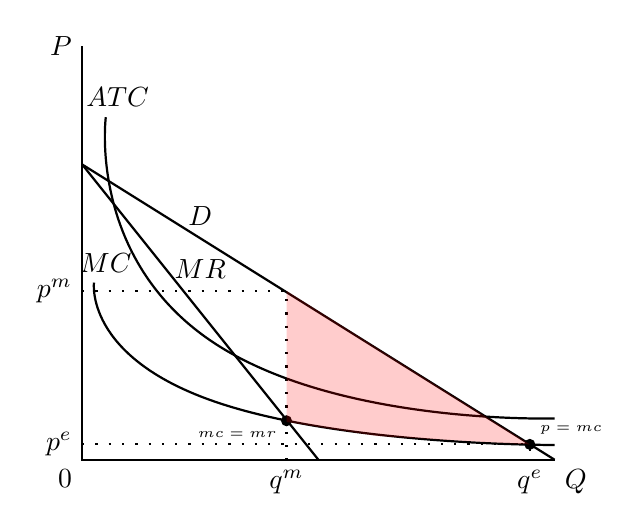
\begin{tikzpicture}[thick,font=\sffamily,scale=1.5]
	%axis
	 \draw (0,3.5) node[left]{$P$} -- (0,0) node[below left] {$0$} 
	  -- (4,0) node[below right]{$Q$};
	  
	\draw[] (0,2.5) -- (4,0); %Demand
	\draw[] (0,2.5) -- (2,0); %MR

	%Iso-profits
	\draw[] plot [smooth, tension=1] coordinates {(0.2,2.9) (1.1,1) (4,0.35)}; %ATC
	\draw[] plot [smooth, tension=1] coordinates {(0.1,1.5) (1.1,0.5) (4,0.125)}; %MC

	
	
	
	%labels
	\node[above] at (0.3,2.9) {$ATC$}; %ATC label
	\node[above] at (0.2,1.5) {$MC$}; %mC label
	\node[above] at (1,1.9) {$D$}; %D label
	\node[above] at (1,1.45) {$MR$}; %MR label
	
	%equilibria labels
	\node[style={fill=black,circle,inner sep=0pt,minimum size=4pt}] at (1.73,0.33) { }; %mc=mr node
	\node[below left]at (1.73,0.33) {\tiny{$mc=mr$}}; %mc=mr label
	\node[style={fill=black,circle,inner sep=0pt,minimum size=4pt}] at (3.79,0.13) { }; %p=mc node
	\node[above right]at (3.79,0.13) {\tiny{$p=mc$}}; %p=mc label
	
	%dotted lines	
	\draw[loosely dotted] (0,1.43) node[left]{$p^{m}$} -| node[pos=0.25,below=3mm] {}
	  (1.73,0) node[below]{$q^{m}$}; %monopoly q dotted lines
	\draw[loosely dotted] (0,0.13) node[left]{$p^{e}$} -| node[pos=0.25,below=3mm] {}
	  (3.79,0) node[below]{$q^{e}$}; %allocatively efficient dotted lines
	  
	  	\fill [fill=red, fill opacity=0.2] (1.73,1.43) node[left]{} -- (1.73,0.32) node[below left] {} -- (2.5,0.2) node[below left] {} -- (3.79,0.13) node[below left] {}; %blue fill (with an intermediate coordinate to make it seem smooth)
\end{tikzpicture}
\end{document}